\documentclass[compress,12pt]{beamer}
\usepackage{caption}
\usepackage{subcaption}
\usetheme{Arguelles}
\usepackage{color}
\usepackage{tcolorbox}
\usepackage{xcolor}
\usepackage{booktabs}
\usepackage{algorithm,algpseudocode}
\usepackage{amsfonts, amsmath, amssymb}
\newcommand{\myRed}[1]{\textcolor{red}{#1}}

\title{MATH 512 - Project 3}
\subtitle{}
\event{}
\date{}
\author{Wasif Ahmed, Haoxiang Deng, Jacob Fein-Ashley, Kanav Malhotra, Longzhe Yang}


\begin{document}

\frame[plain]{\titlepage}

\section{Question 1}



\begin{frame}{Question 1 Overview}
      \begin{itemize}
            \item Let $W_t$ be a standard Wiener process, with drift parameter zero and variance parameter $\sigma^2 = 1$.
            \item We divide the interval $[0,2]$ into $L$ subintervals $[t_i, t_{i+1}]$, where $t_i = i\delta t$ and $\delta t = 2/L$.
            \item Let $W_i = W(t_i)$ and $\delta W_i = W_{i+1} - W_i$.
            \item We verify numerically that:
            \begin{itemize}
                  \item $\sum_{i=0}^{L-1} |\delta W_i|$ is unbounded as $\delta t$ goes to zero.
                  \item $\sum_{i=0}^{L-1} \delta W_i^2$ converges to 2 in probability as $\delta t$ goes to zero.
            \end{itemize}
      \end{itemize}
      
\end{frame}

\begin{frame}{Question 1 Response}
      Refer to Figure~\ref{fig:convergence1}

      \begin{figure}[H]
      \centering
      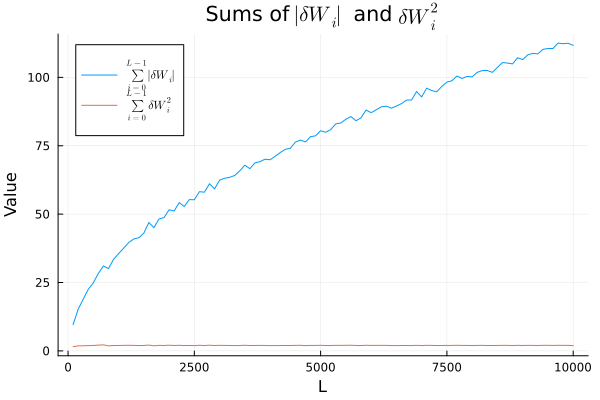
\includegraphics[scale=0.32]{imgs/convergence1.png}
      \caption{Stochastic Plots}
      \label{fig:convergence1}
      \end{figure}

Notice that as the $L$ parameter increases, the $|\delta W_i|$ term is unbounded while $\delta W_i^2$ converges to $2$ in probability.
\end{frame}
\section{Question 2}
\begin{frame}{Question 2a}

      \begin{figure}[H]
            \centering
            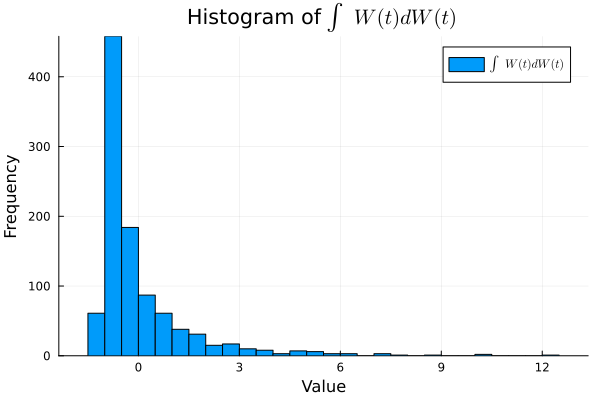
\includegraphics[scale=0.5]{imgs/2a.png}
            \caption{2a}
            \label{fig:2a}
      \end{figure}

\end{frame}

\begin{frame}{Question 2b}

      \begin{figure}[H]
            \centering
            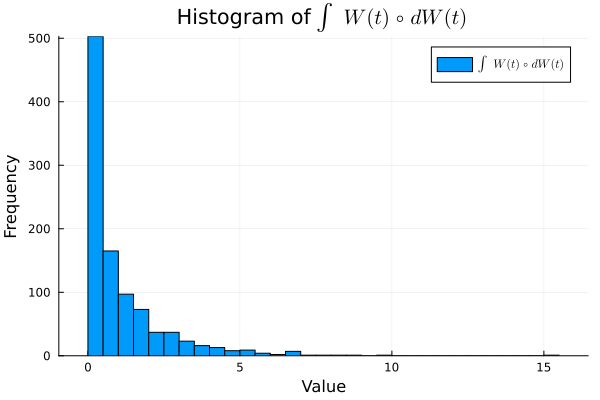
\includegraphics[scale=0.5]{imgs/2b.png}
            \caption{2b}
            \label{fig:2b}
      \end{figure}
\end{frame}

\begin{frame}{Question 2c}

      \begin{figure}[H]
            \centering
            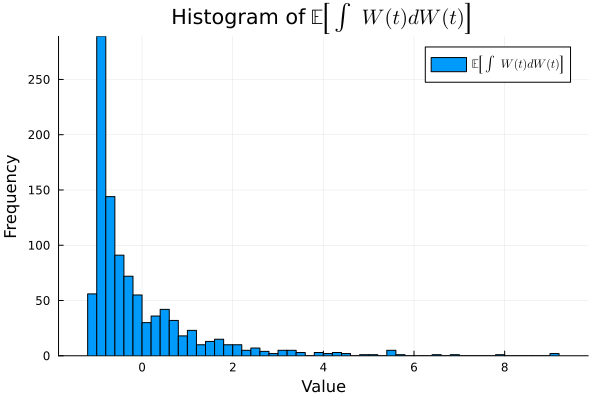
\includegraphics[scale=0.5]{imgs/2c.png}
            \caption{2c}
            \label{fig:2c}
      \end{figure}
\end{frame}


\begin{frame}{Question 2d}
      \begin{figure}[H]
            \centering
            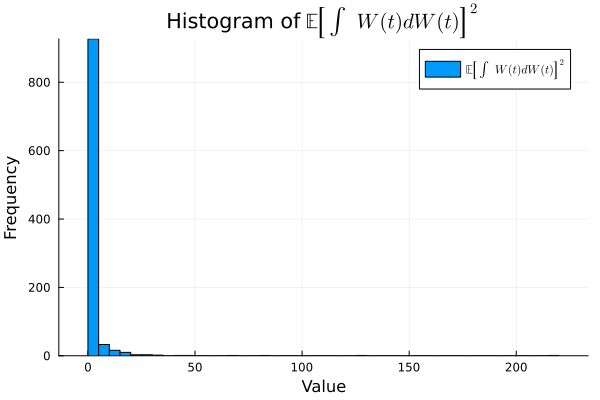
\includegraphics[scale=0.5]{imgs/2d.png}
            \caption{2d}
            \label{fig:2d}
      \end{figure}
\end{frame}


\begin{frame}{Question 2e}
      \begin{figure}[H]
            \centering
            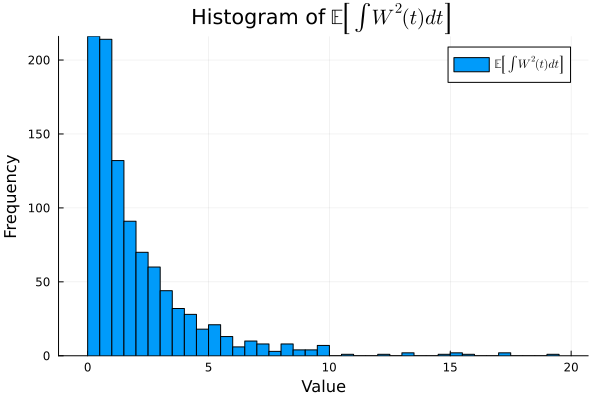
\includegraphics[scale=0.5]{imgs/2e.png}
            \caption{2e}
            \label{fig:2e}
      \end{figure}

\end{frame}

\begin{frame}{Question 2f}
      \begin{figure}[H]
            \centering
            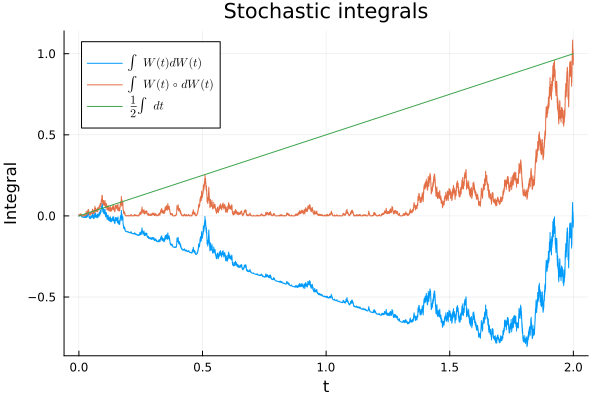
\includegraphics[scale=0.5]{imgs/2f.png}
            \caption{2f}
            \label{fig:2f}
      \end{figure}

\end{frame}

\section{Question 3}
\begin{frame}{Question 3: Weak and Strong Order of Convergence for EM Method}

    \textbf{Objective:} Analyze the weak and strong order of convergence of the Euler-Maruyama method for solving the given Stochastic Differential Equation (SDE):
    \[
    dX(t) = \mu X(t) dt + \sigma X(t) dW(t), \quad X(0)=3, \quad \mu=2 , \quad \sigma=0.10
    \]

    \begin{itemize}
        \item \textbf{Weak order of convergence equal to 1}, indicating that the error in the expected value of the solution does not converge with the decrease of time step size, \(\Delta t\).
        \item \textbf{Strong order of convergence equal to 0.5:}, meaning that the expected value of the absolute error between the numerical and exact solutions decreases with the square root of the time step size.
    \end{itemize}
\end{frame}

\begin{frame}{Weak Order of Convergence Results}
    \textbf{Findings:} Through MATLAB simulations over various \(\Delta t\), we observed:
    
    \begin{itemize}
        \item A plot of the error versus \(\Delta t\) for the  weak order of convergence of 1. 
        \begin{figure}[H]
            \centering
            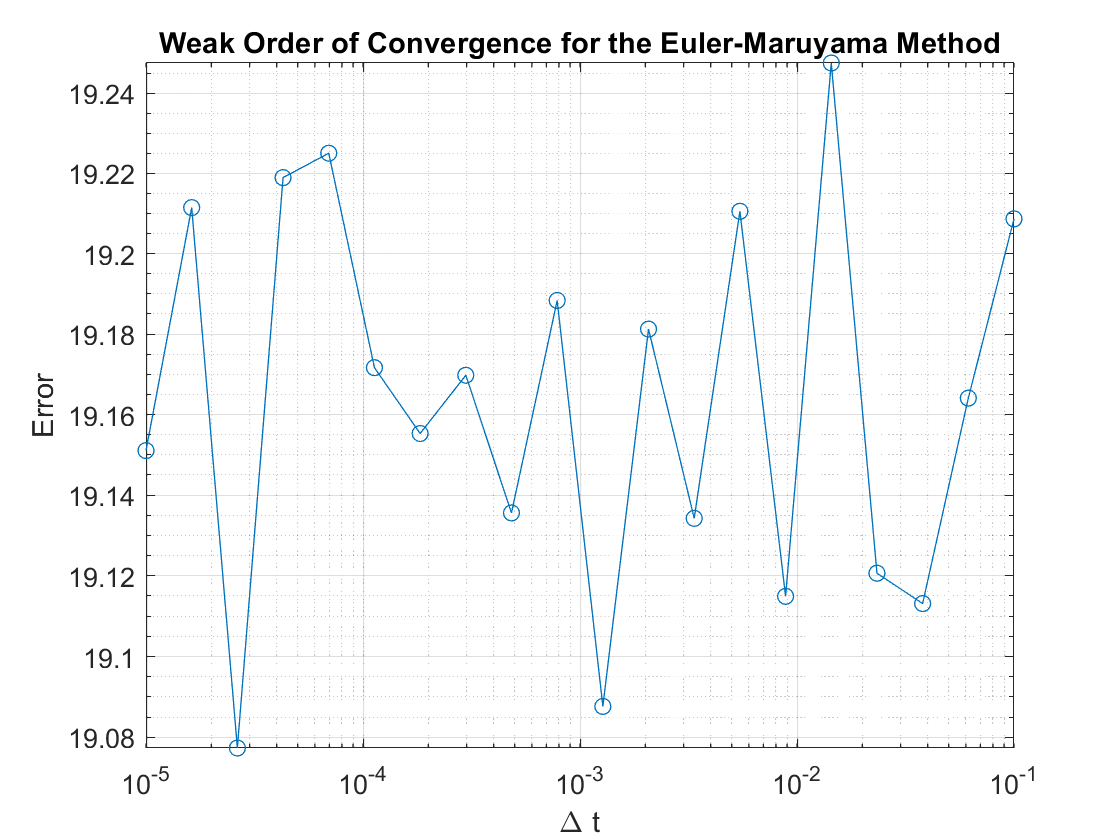
\includegraphics[scale=0.25]{project4Q3fig1.png}
            \label{fig:3a}
       \end{figure}
        
    \end{itemize}
\end{frame}

\begin{frame}{Strong Order of Convergence Results}
    \textbf{Findings:} For the strong order of convergence:
    
    \begin{itemize}
        \item A strong order of convergence of \(0.5\). 
          % Use the minipage environment to place figures side by side
            
            \begin{minipage}{0.4\textwidth}
            \begin{figure}
                \centering
                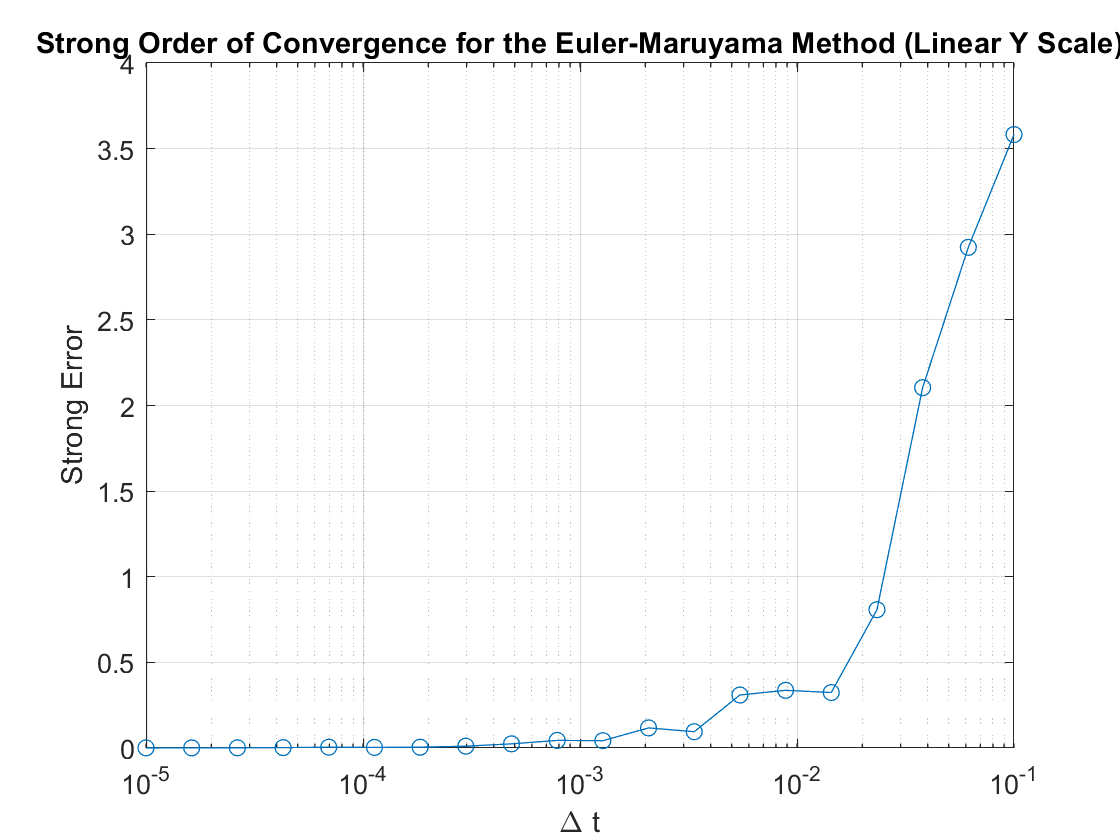
\includegraphics[width=\linewidth]{project4Q3fig3.png} % Adjust the 
                \caption{Weak Order of Convergence}
                \label{fig:enter-label}
            \end{figure}
            \end{minipage}%
            \hfill % This adds space between the figures if needed
            \begin{minipage}{0.4\textwidth}
            \begin{figure}
                \centering
                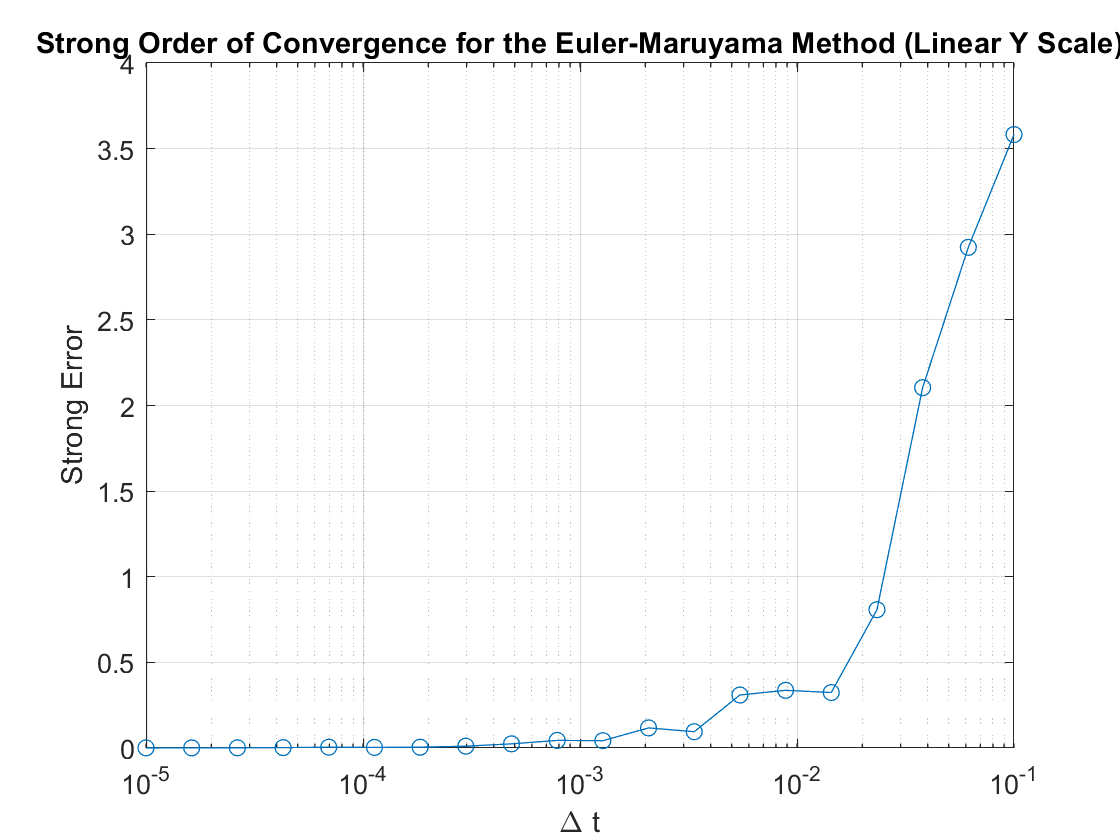
\includegraphics[width=\linewidth]{project4Q3fig3.png} % Adjust the 
                \caption{Strong Order of Convergence}
                \label{fig:enter-label}
            \end{figure}
                
            \end{minipage}
    \end{itemize}
    
    \textbf{Note:} These results show the Euler-Maruyama method has a weak order of convergence equal to 0.5 and a strong order of convergence equal to 1.
\end{frame}

\section{Question 4}
\begin{frame}{Question 4}
      % # Consider the following SDE:
      % # 𝑑𝑋(𝑡) = 𝜇𝑋(𝑡)𝑑𝑡 + 𝜎𝑋(𝑡)𝑑𝑊(𝑡) , 𝑋(0) = 3, 𝜇 = 2 , 𝜎 = 0.10
      % # a) Simulate (over the interval [0,20]) this stochastic process using an implicit method of the form
      % # 𝑋𝑛+1 = 𝑋𝑛 + (1 − 𝜃)𝛥𝑡𝑓(𝑋𝑛) + 𝜃𝛥𝑡𝑓(𝑋𝑛+1) + √𝛥𝑡𝛼𝑛𝑔(𝑋𝑛)

      We consider the following SDE:
      \[
      dX(t) = \mu X(t) dt + \sigma X(t) dW(t), \quad X(0)=3, \quad \mu=2 , \quad \sigma=0.10
      \]

      \begin{itemize}
            \item Simulate this stochastic process over the interval $[0,20]$ using an implicit method of the form:
            \[
            X_{n+1} = X_n + (1 - \theta) \Delta t f(X_n) + \theta \Delta t f(X_{n+1}) + \sqrt{\Delta t} \alpha_n g(X_n)
            \]
            \item We use $\theta = 0.5$ and $\alpha_n = \sigma X_n$.
            \item We plot the results for $\Delta t = 0.01$ and $\Delta t = 0.001$.
      \end{itemize}

\end{frame}

\begin{frame}{Question 4 Continued}
      We plot the explicit and implicit methods for $\Delta t = 0.01$ and $\Delta t = 0.001$:
      \begin{figure}[H]
            \centering
            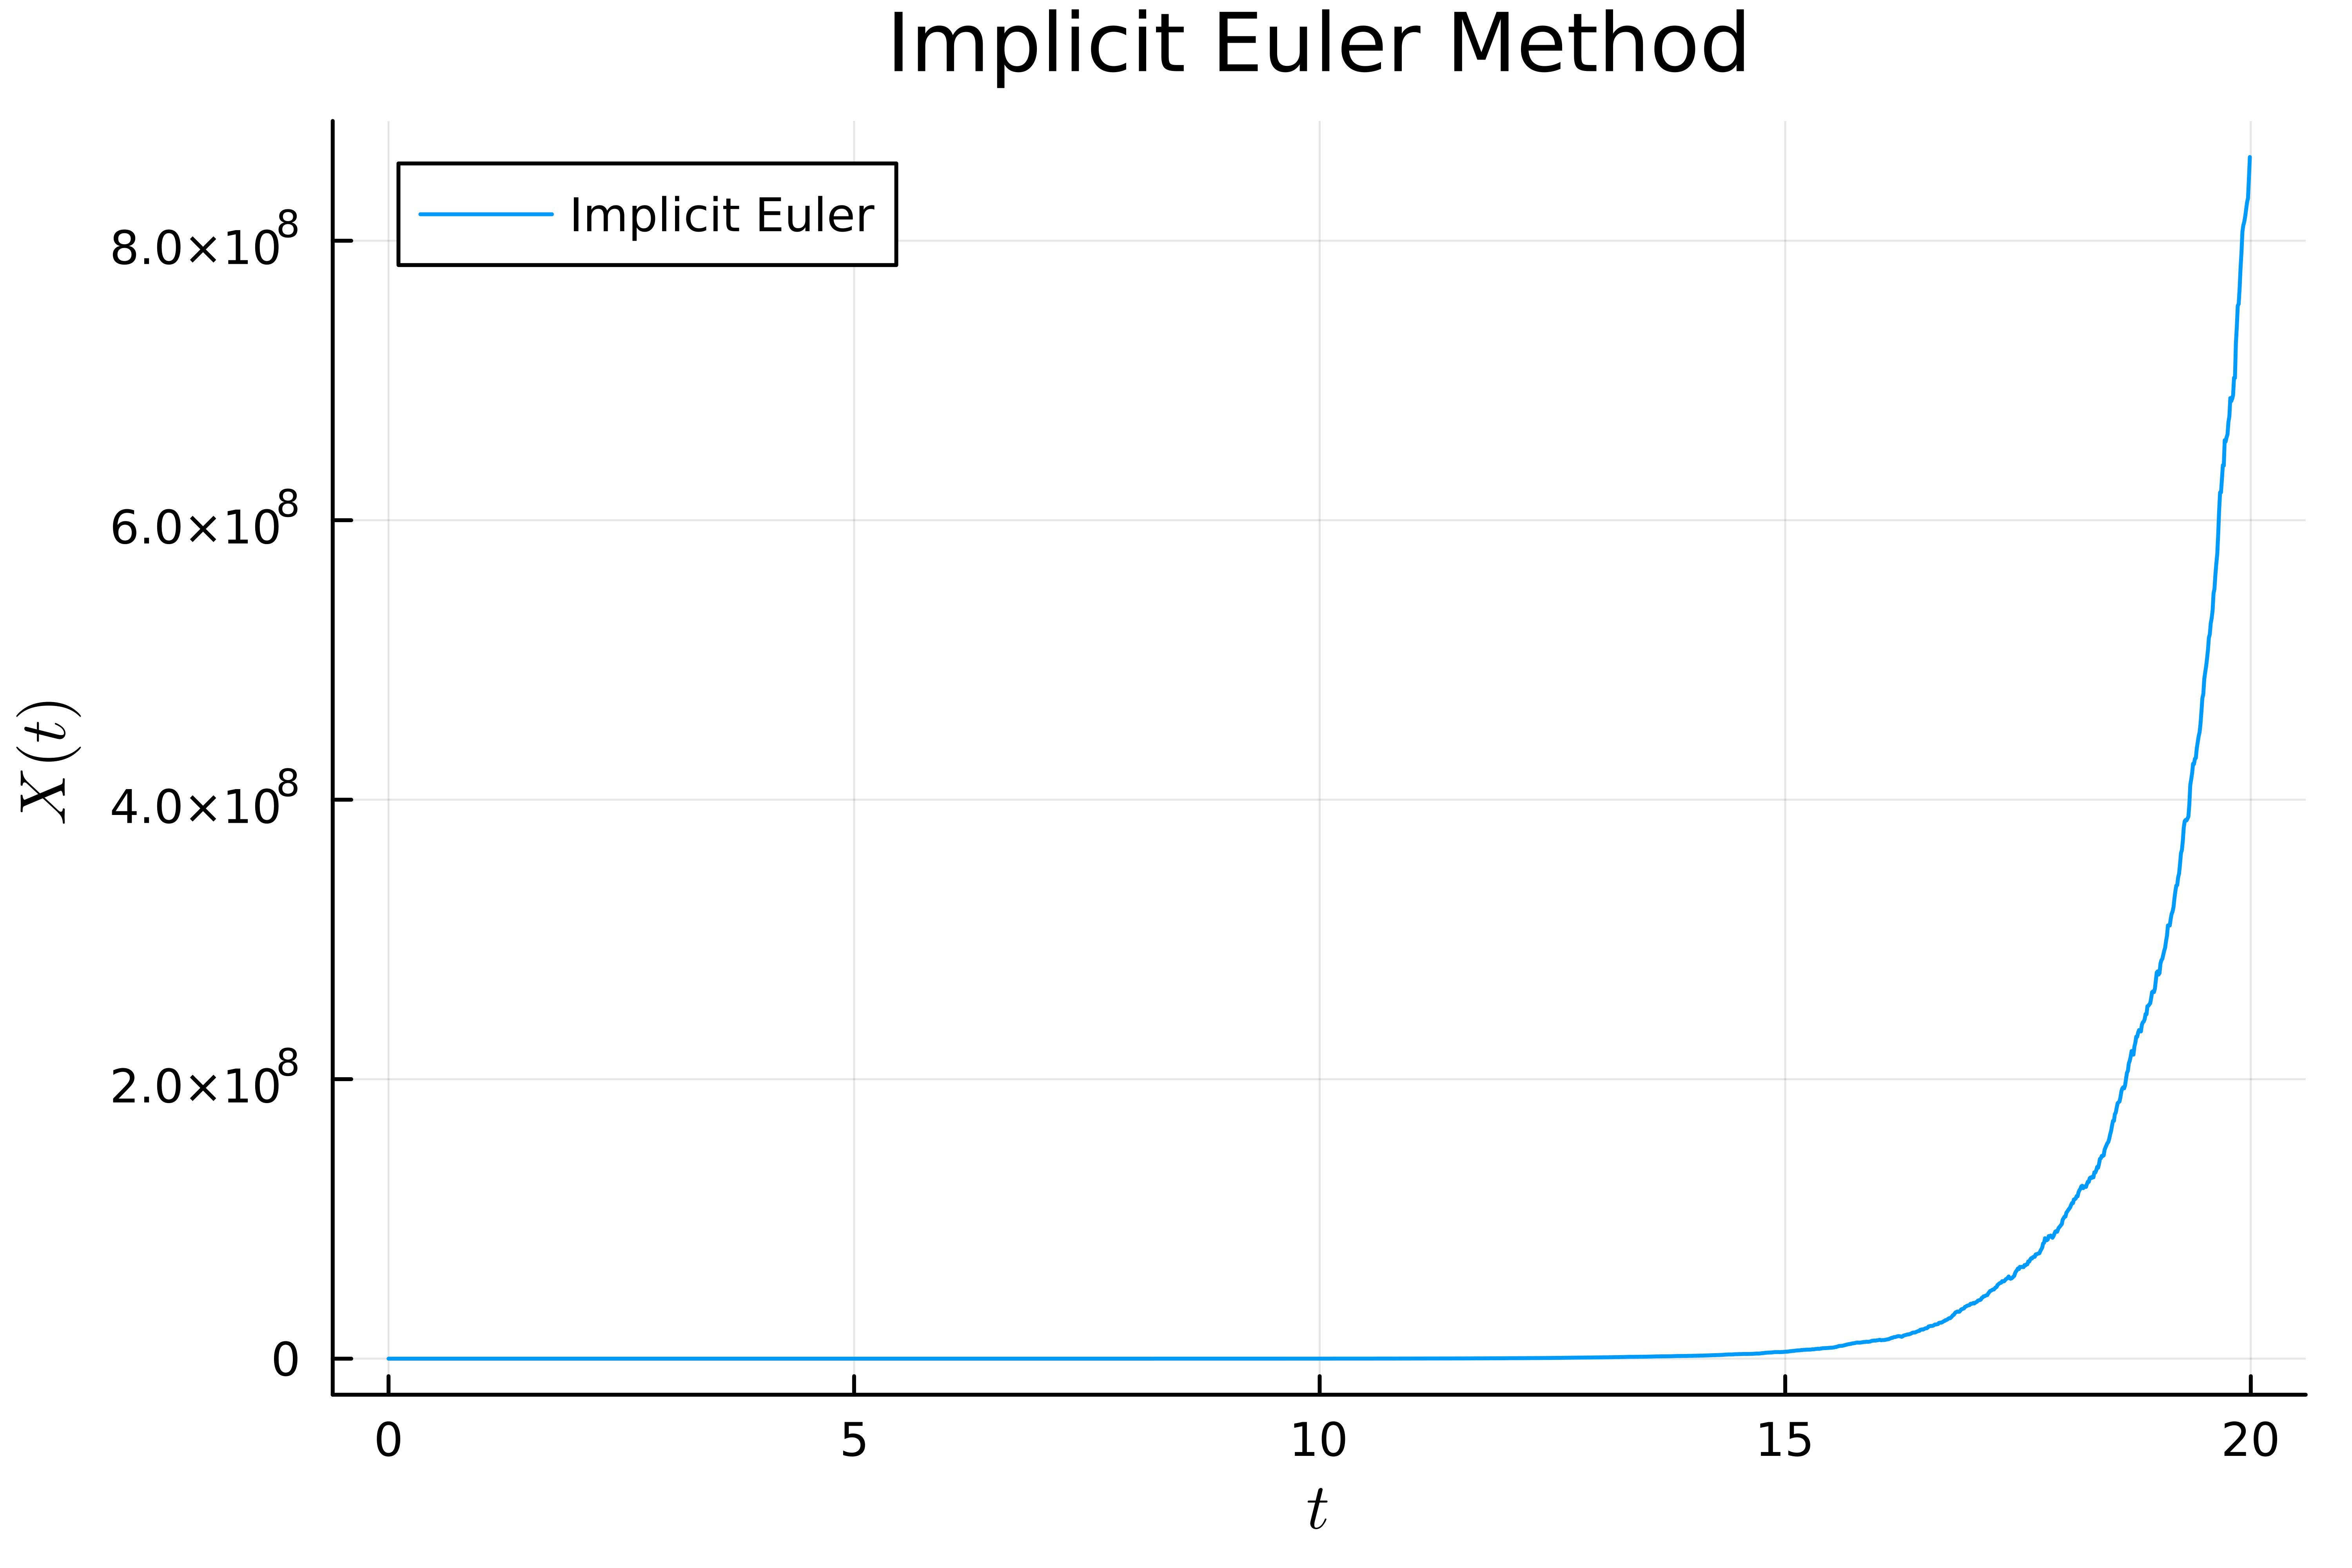
\includegraphics[scale=0.04]{imgs/4implicit_euler.png}
            \caption{Implicit Euler Method}
            \label{fig:4a}
      \end{figure}
\end{frame}

\begin{frame}{Question 4 Continued}
      \begin{figure}[H]
            \centering
            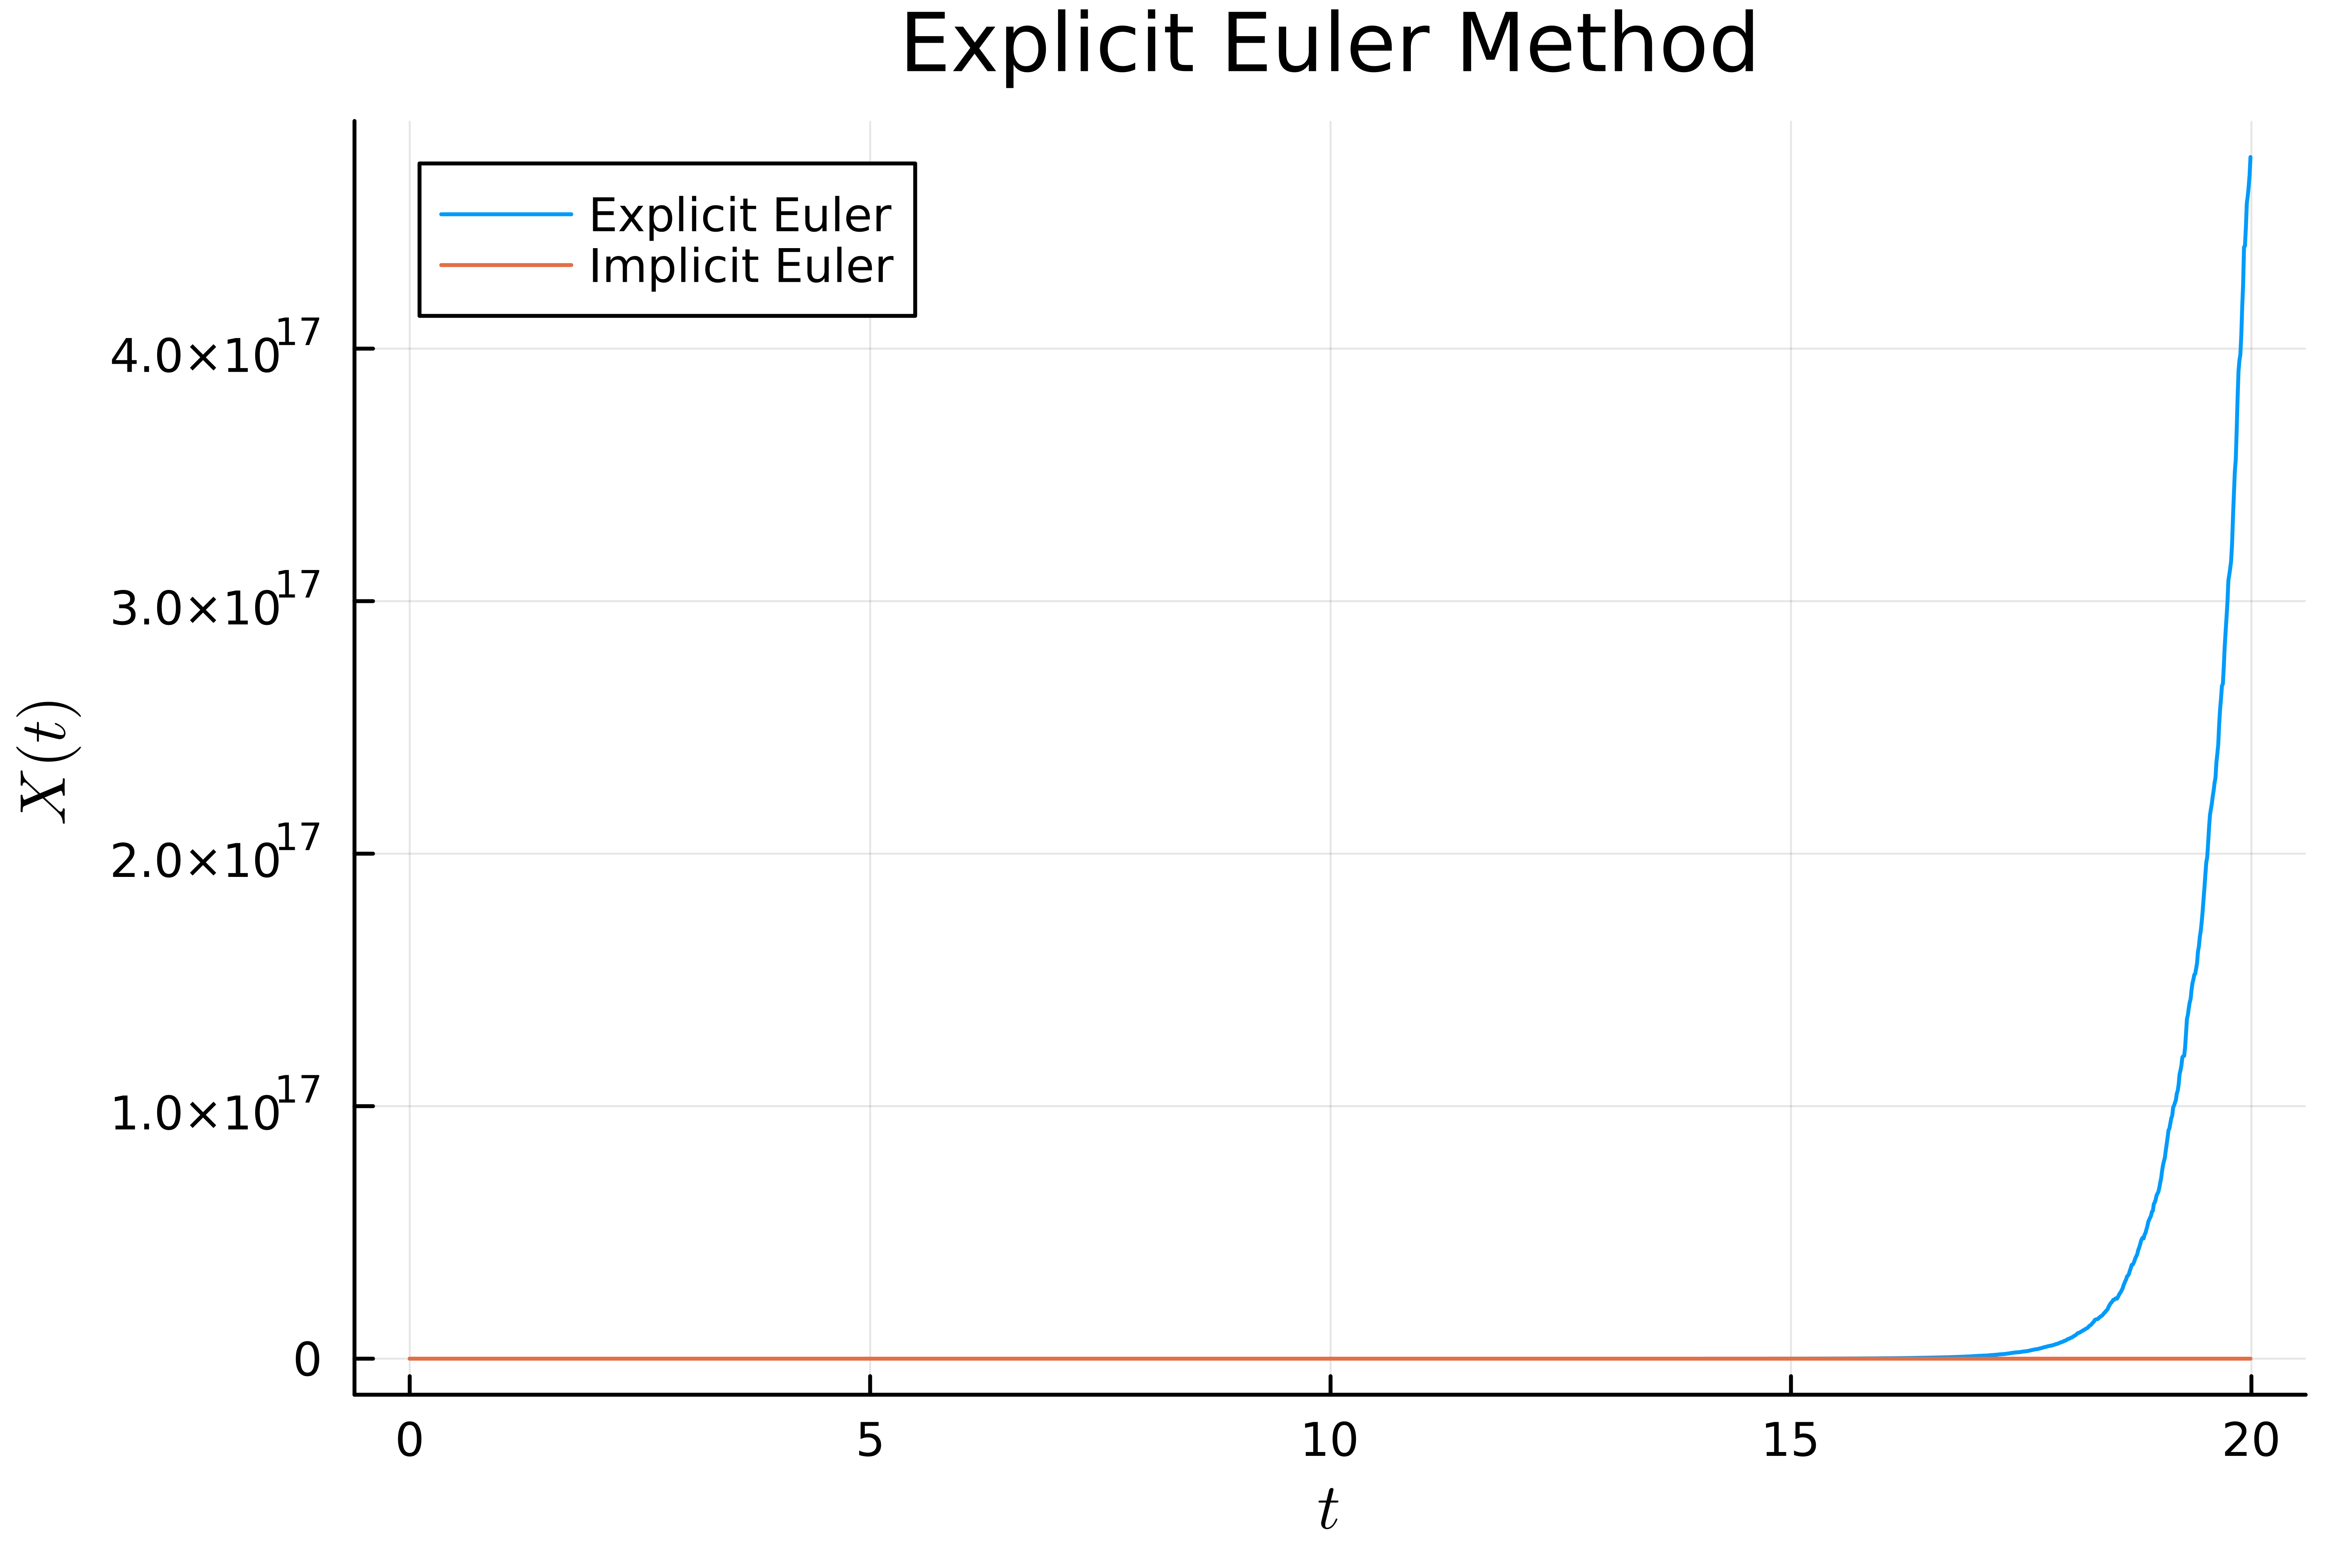
\includegraphics[scale=0.04]{imgs/4explicit_euler.png}
            \caption{Explicit Euler Method}
            \label{fig:4b}
      \end{figure}
\end{frame}

\begin{frame}{Question 4 Continued}
      % c) For what values of 𝜇 𝑎𝑛𝑑 𝜎 is the SDE mean-square stable.
      We determine the values of $\mu$ and $\sigma$ for which the SDE is mean-square stable:
      \begin{figure}
            \centering
            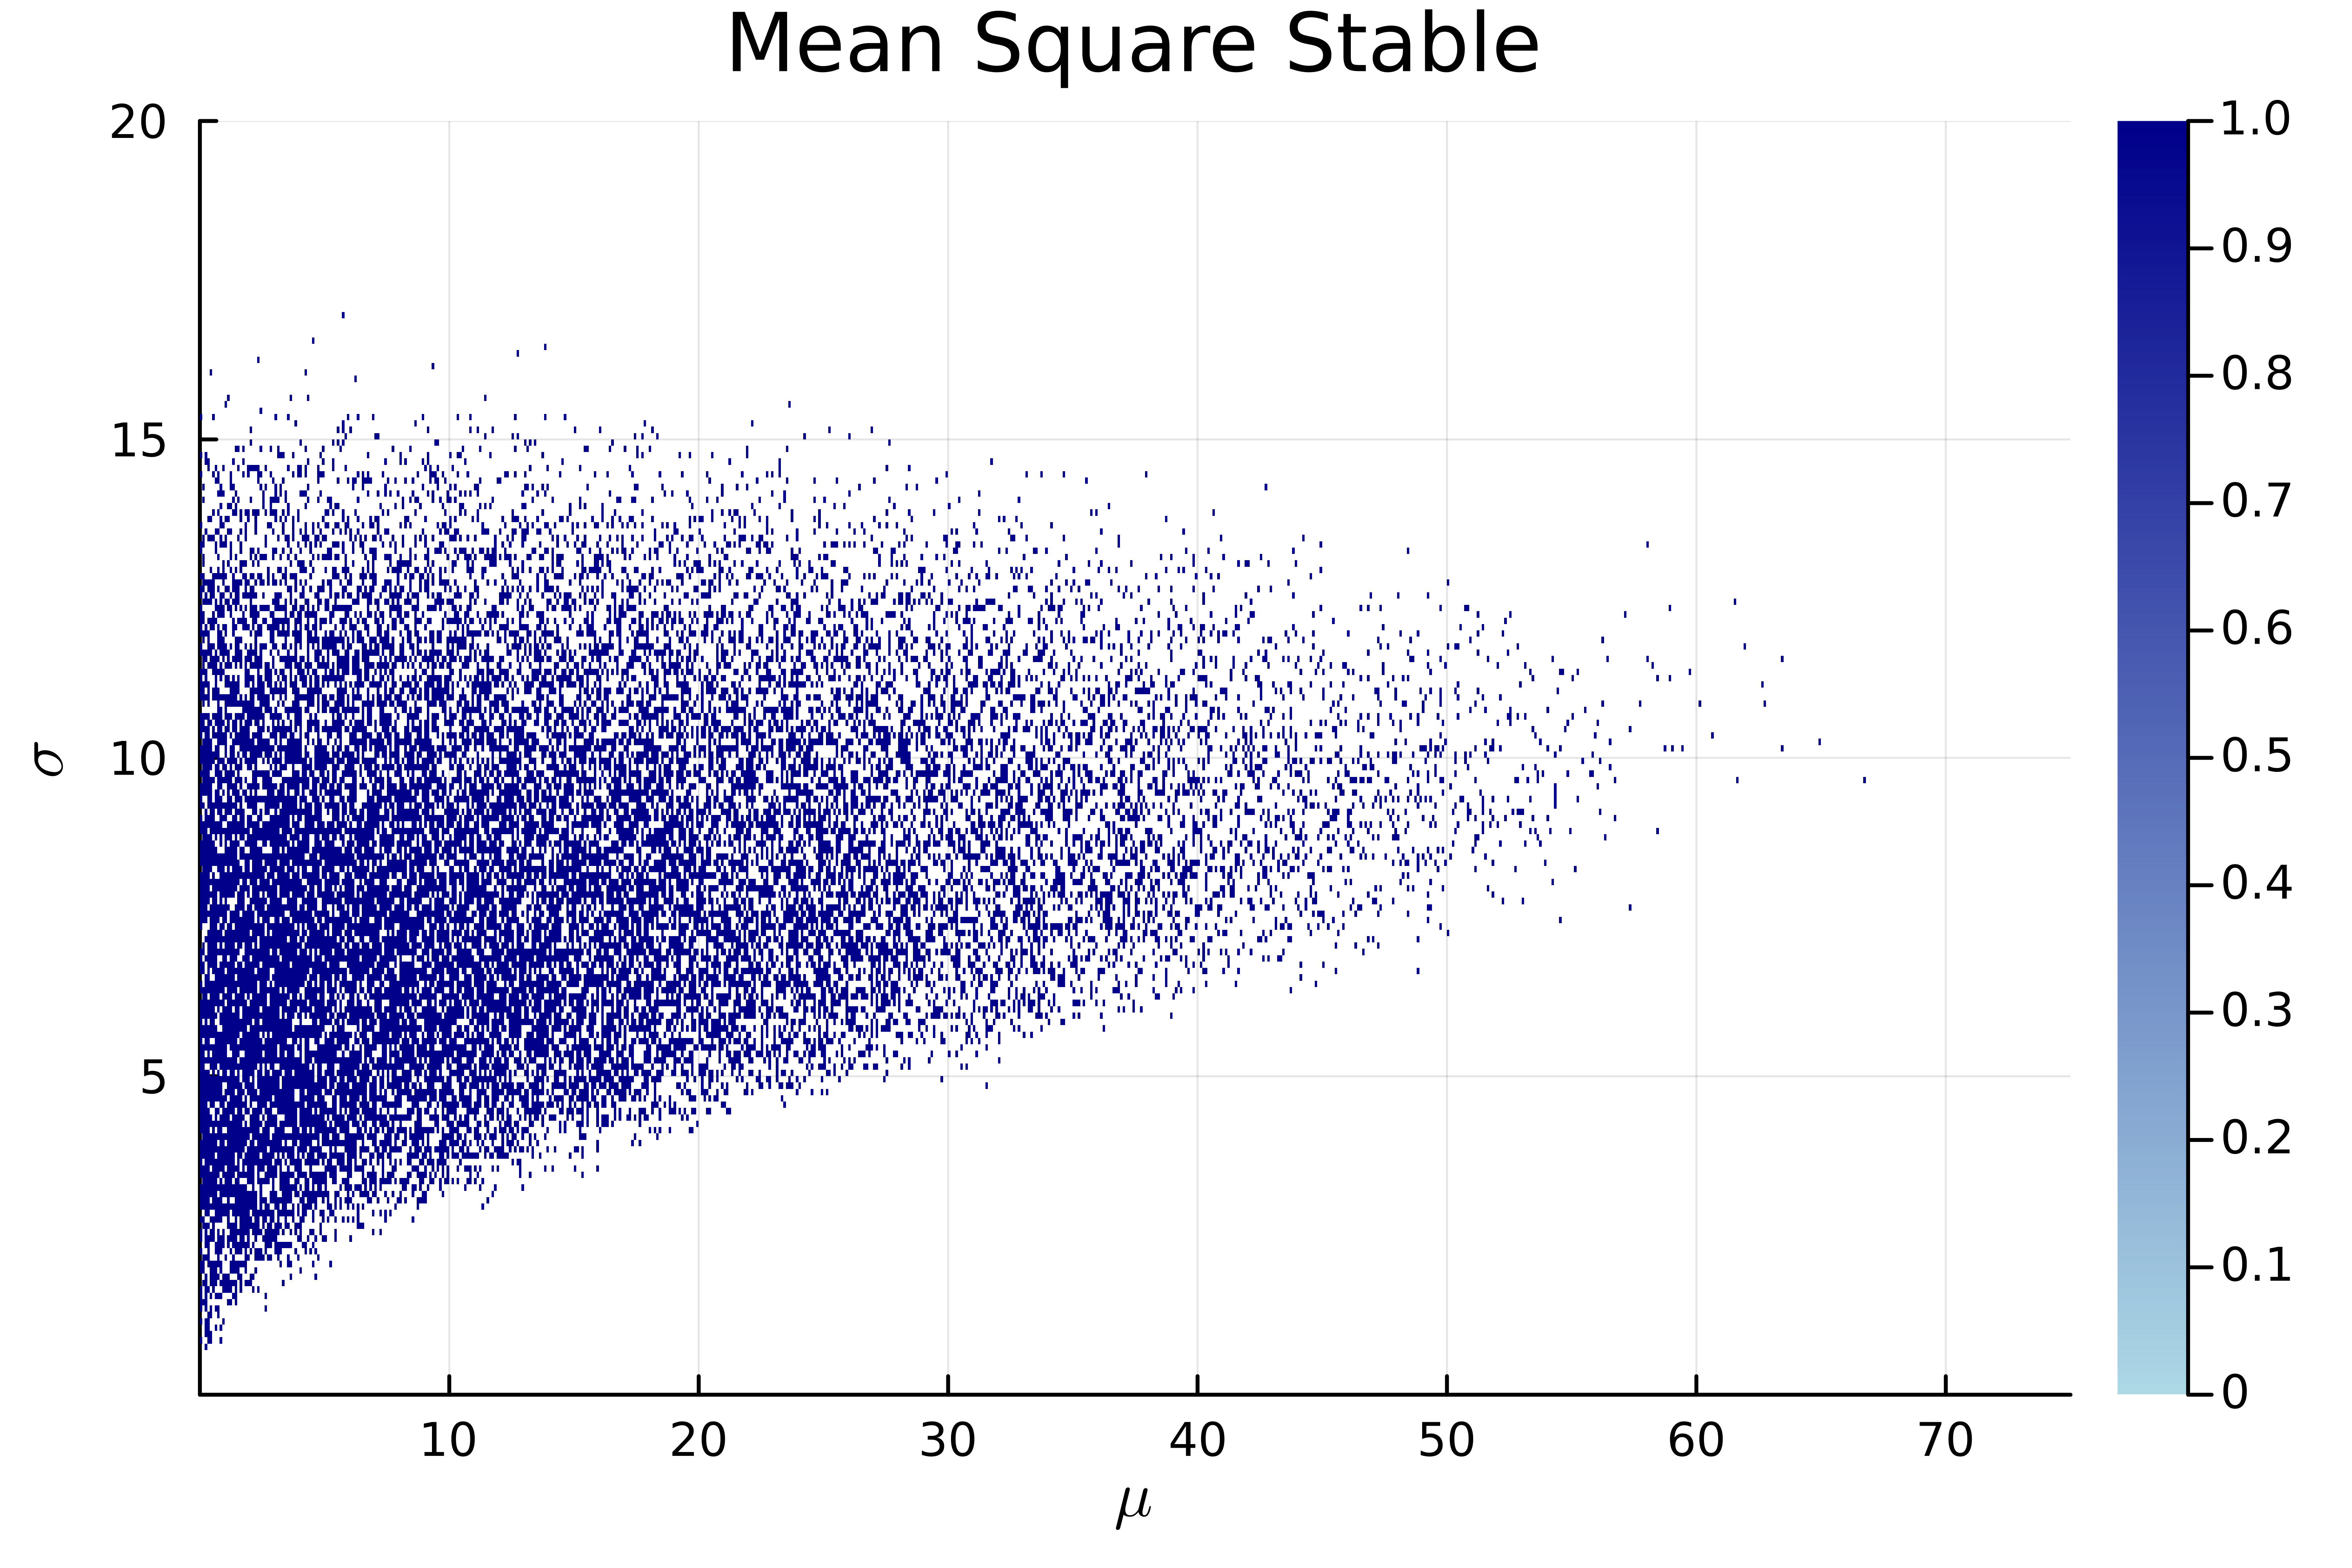
\includegraphics[scale=0.03]{imgs/4mean_square_stable.png}
            \caption{Mean-Square Stability}
            \label{fig:4c}
      \end{figure}
      and we find that the SDE is not mean square stable for any values of $\theta$.
\end{frame}



\section{Question 5}
\begin{frame}{Question 5}
An algorithm to simulate exit times for the SDE:
\begin{algorithmic}[1]
    \State Choose a step size $\Delta t$
    \State Choose a number of paths, $M$
    \For{$s = 1$ to $M$}
        \State Set $t_n = 0$ and $X_n = X_0$
        \While{$X_n > a$ and $X_n < b$}
            \State Compute a $N(0,1)$ sample $\xi_n$
            \State Replace $X_n$ by $X_n + \Delta t f(X_n) + \sqrt{\Delta t} \xi_n g(X_n)$
            \State Replace $t_n$ by $t_n + \Delta t$
        \EndWhile
        \State Set $T_s^{exit} = t_n - 1/2 \Delta t$
    \EndFor
    \State Set $a_M = \frac{1}{M} \sum_{s=1}^{M} T_s^{exit}$
    \State Set $b^2_M = \frac{1}{M-1} \sum_{s=1}^{M} (T_s^{exit} - a_M)^2$
\end{algorithmic}
\end{frame}

\begin{frame}{Question 5 Continued}
      \begin{figure}[H]
            \centering
            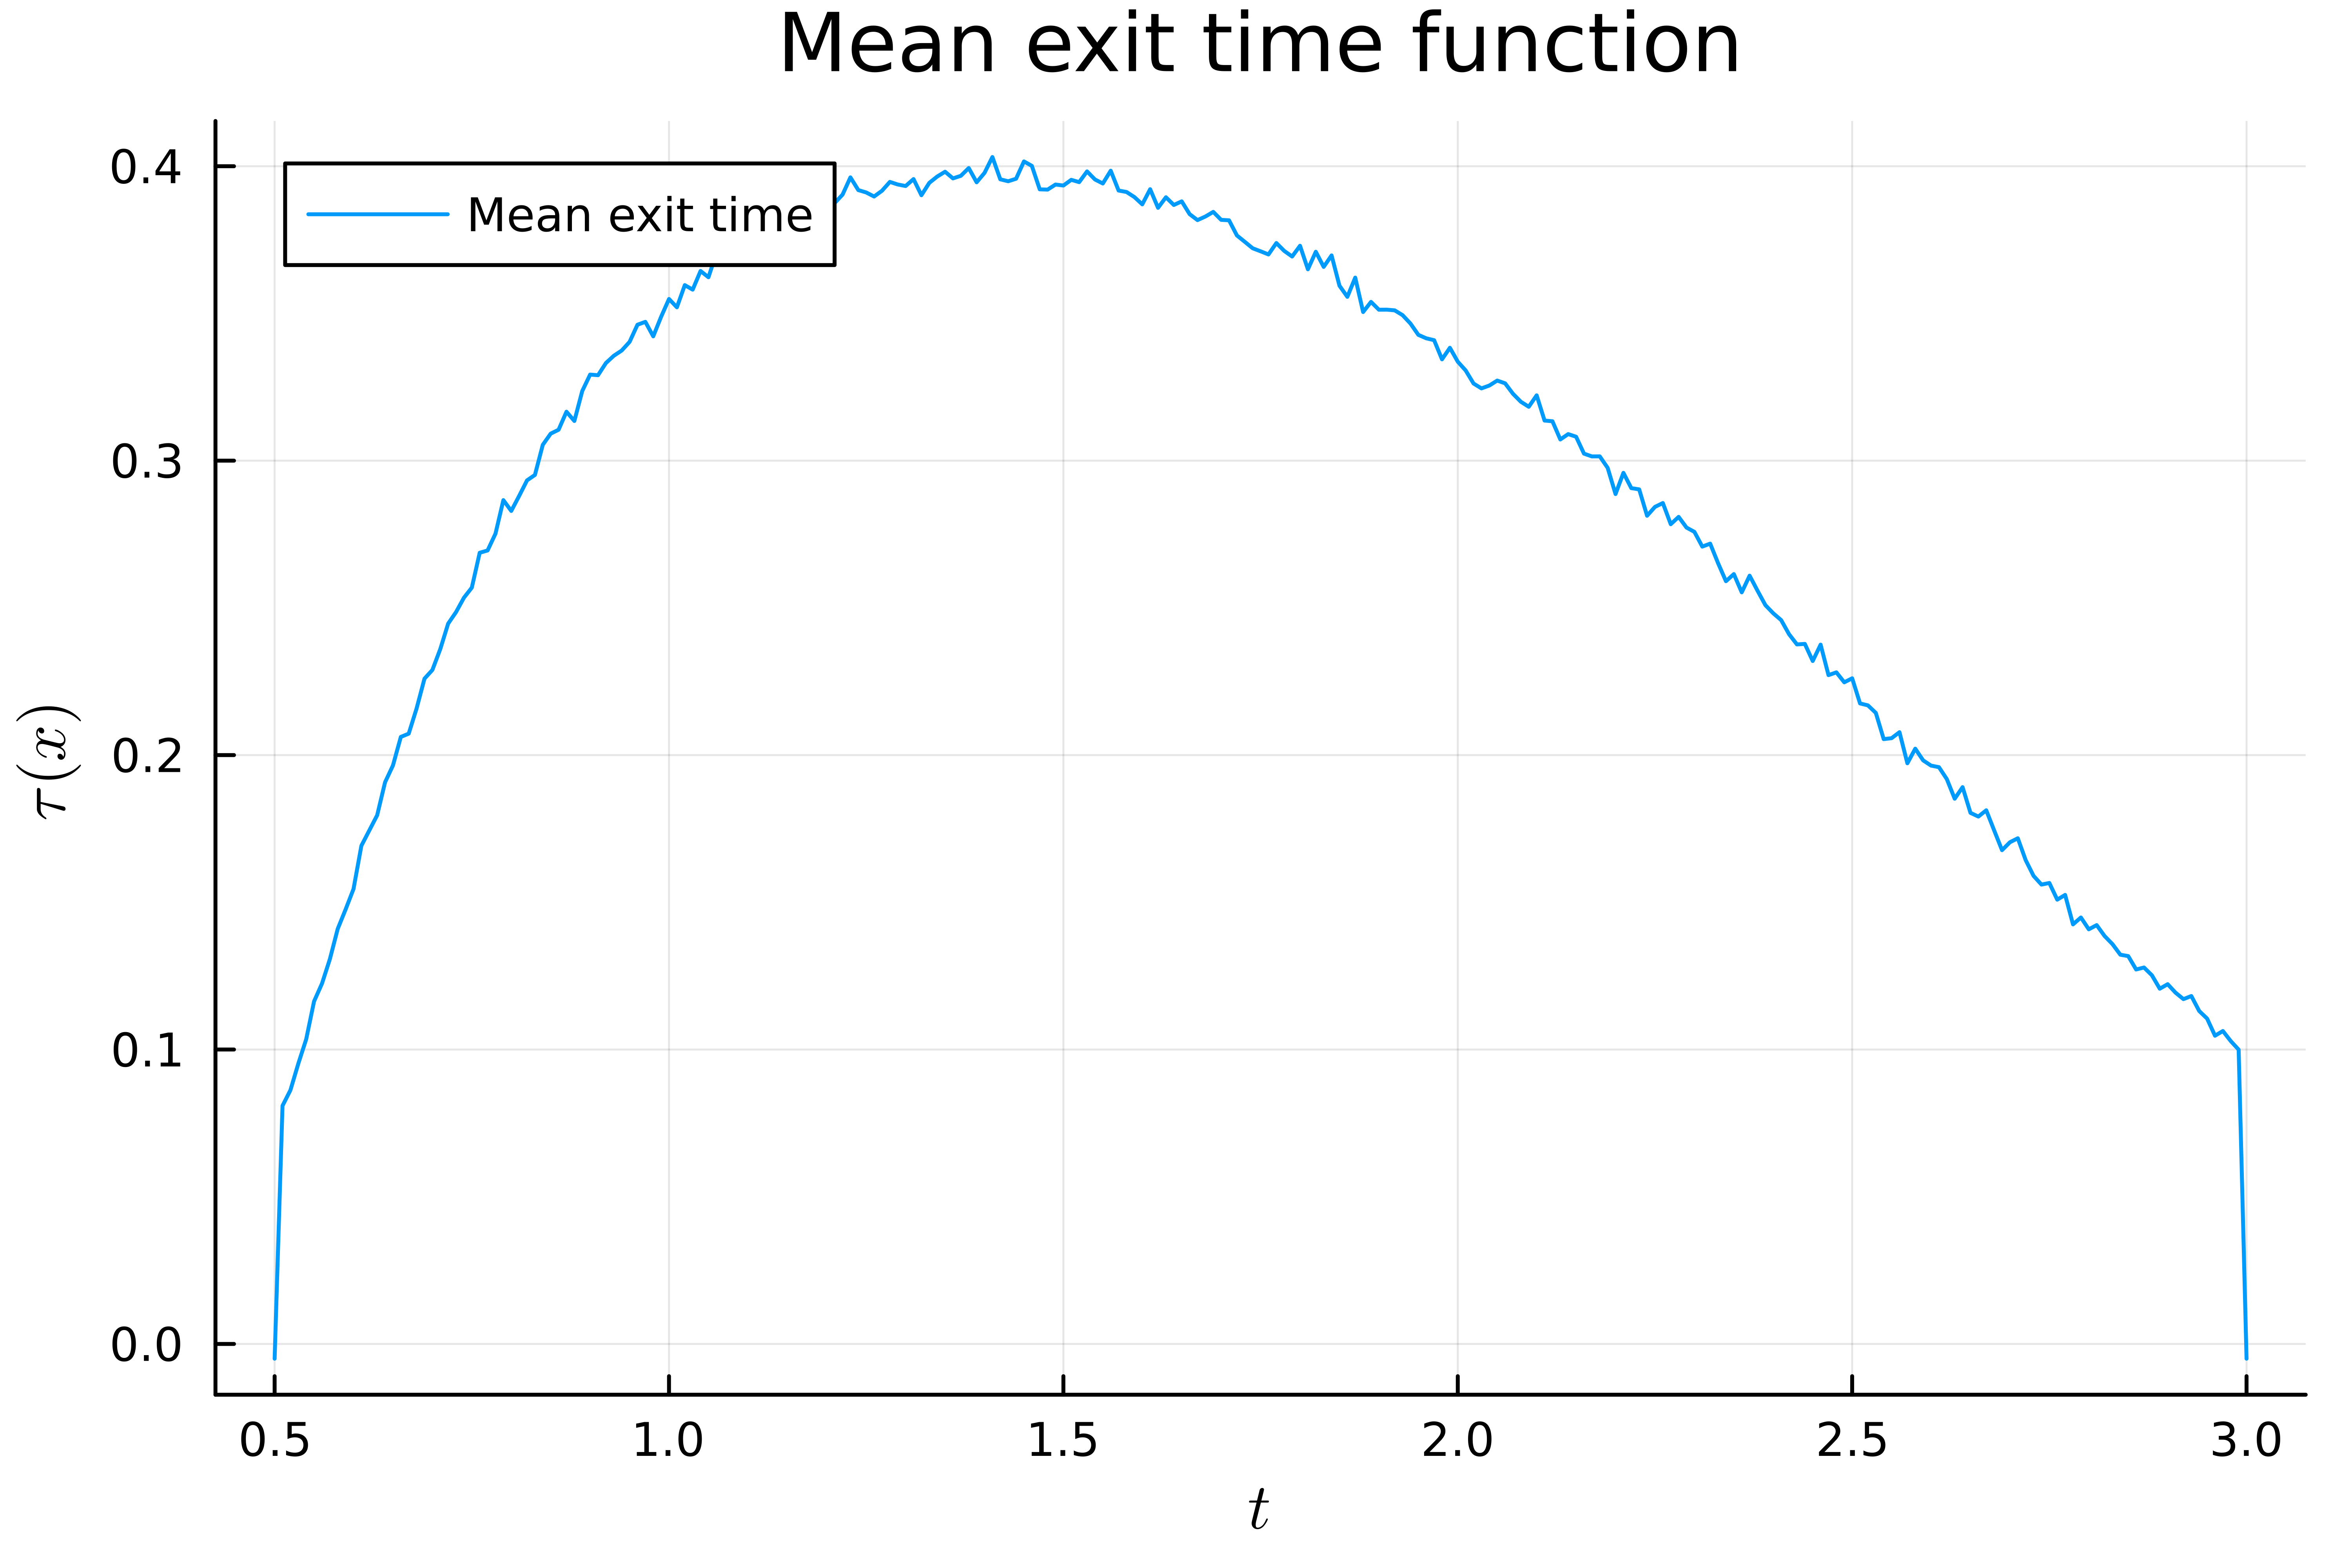
\includegraphics[scale=0.05]{imgs/5mean_exit_time.png}
            \caption{5}
            \label{fig:5}
      \end{figure}
\end{frame}

\begin{frame}{Question 5 Continued}
      \begin{figure}[H]
            \centering
            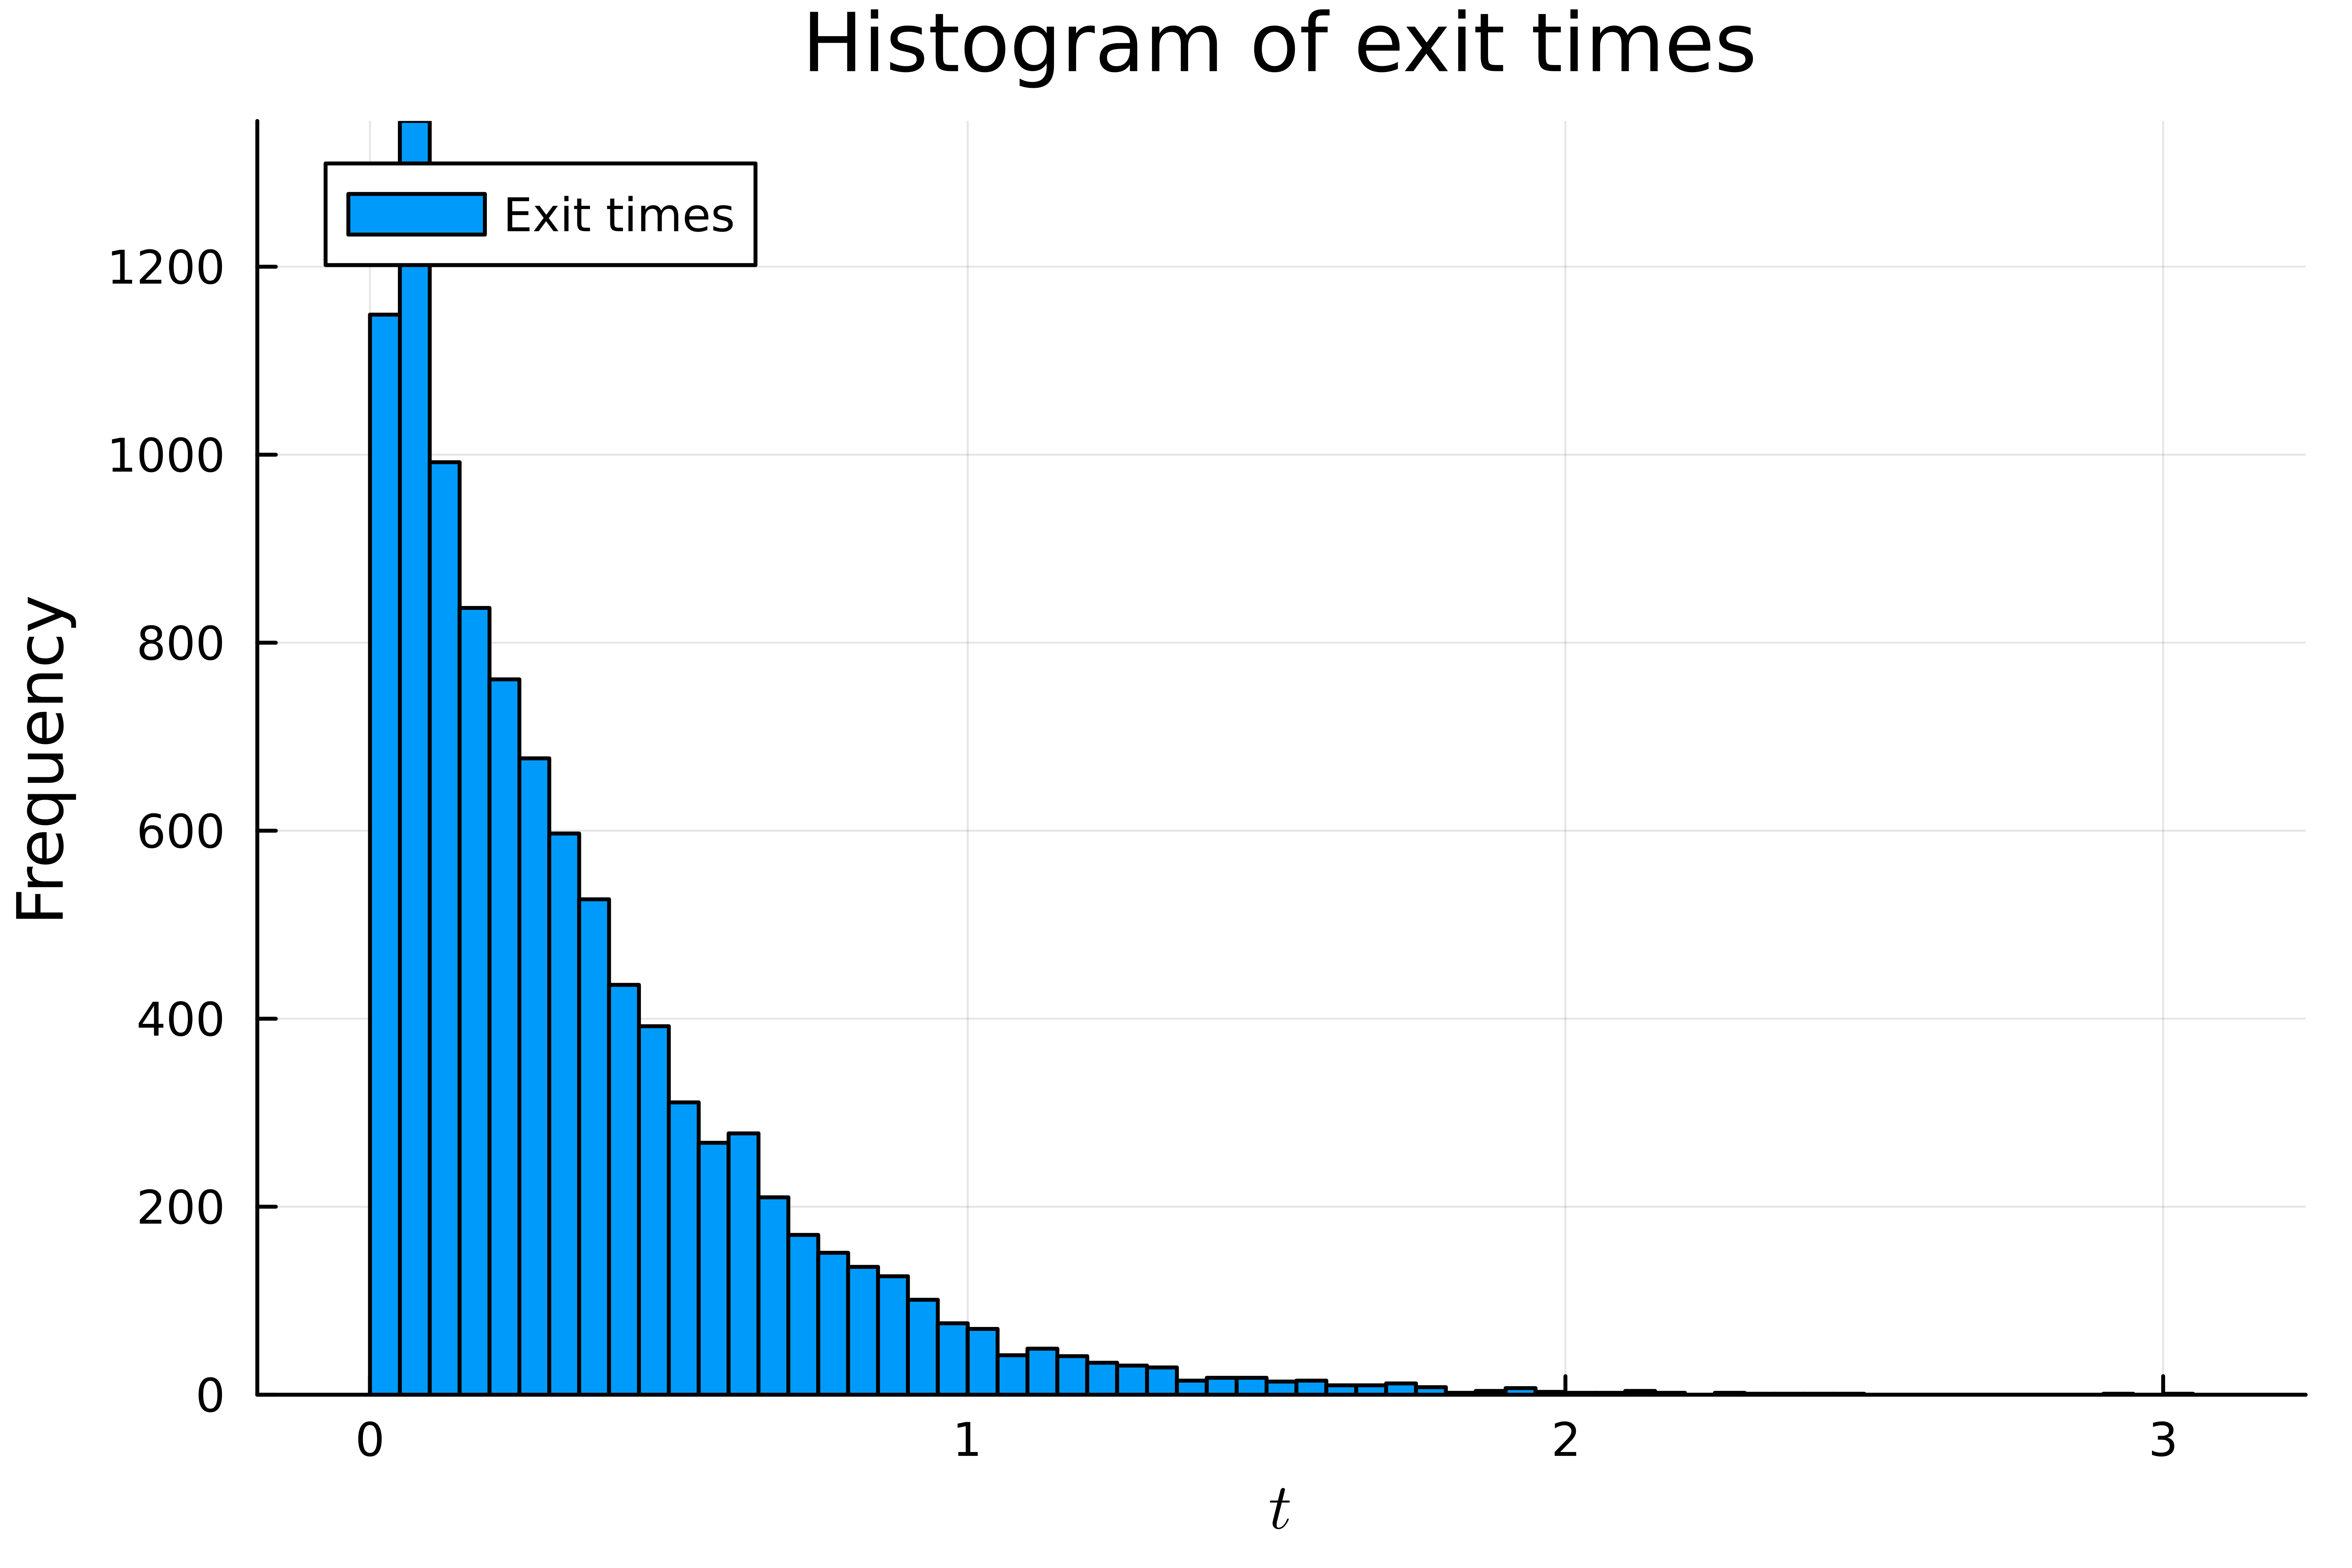
\includegraphics[scale=0.05]{imgs/5exit_times_histogram.png}
            \caption{5}
            \label{fig:5_exittimeshist}
      \end{figure}
\end{frame}

\End
\begin{frame}[plain,standout]
      \centering
      Questions?
\end{frame}

\end{document}

